% =====================================================================
% File: chapters/2.Literature-review.tex
% Status: Replaces the master placeholder. Builds on but rewrites the
%         project work literature review (Leonsen 2025) and adds
%         dedicated sections on swirling flow in 90 degree bends, on
%         the RPT-side cavitation/pre-rotation literature relevant to
%         the booster concept, and on the booster--RPT system context
%         that the master thesis works inside.
% =====================================================================
\chapter{Literature review}
\label{chap:chap2}
 
\begin{center} % Abstract overview
\singlespacing\parbox{12cm}{\textit{
This chapter reviews the literature that the master thesis builds on. The selection follows the order in which the research questions are posed in Chapter~\ref{chap:chap1}: first what previous booster--RPT studies have established and what they have left open, then the multi-objective design tradition that frames the screening campaign, then the hubless rim-driven thruster wake as the design input, the sensitivity of the downstream RPT to pre-rotation, the secondary-flow physics of $90^\circ$ bends, the cascade theory needed to close the design problem, the numerical framework adopted for the simulations, and finally the rotor--stator interaction theory used in the unsteady analysis. The chapter ends with a synthesis that identifies the specific gap this thesis closes.
}}
\end{center}
 
\section{Booster--RPT systems: what previous studies leave open}
\label{sec:lit_booster_open}
 
The cavitation barrier on RPT retrofits has been recognised for at least a decade in the Norwegian hydropower research community~\cite{DagsvikStorli2021, DagsvikThesis2024, Kerlefsen2025}, and the basic case for a booster pump in the draft tube is now well established. Valstad~\cite{Valstad2018} demonstrated for the Roskrepp plant that a dedicated axial booster in series with the RPT raises the pump-mode inlet pressure to a safe level while preserving overall operability of the simplified waterway model. The follow-up studies of contra-rotating axial boosters by Hage~\cite{Hage2020} and Dahle~\cite{Dahle2019} confirmed that the necessary head increase is mechanically achievable. They also reported a less encouraging finding: the cavitation margin and the global efficiency are sensitive to \emph{how} the booster delivers the flow to the RPT, not only to how much head it adds. Strong residual swirl and radially non-uniform discharge profiles measured downstream of contra-rotating boosters were associated with low hydraulic efficiency in tightly constrained installations~\cite{Dahle2019}, and similar observations are reported in the early Store2Hydro RDT studies~\cite{Verdijck2025, Fjuk2025, Ambjornsson2025}.
 
Two limitations recur across these earlier booster studies. First, the analyses treat the booster--RPT pair as a system but do not address what should happen between the two machines. The flow leaving the booster is taken as it is, and the RPT receives it. There is no \emph{element} placed in the gap to condition the flow. Second, where individual designers have considered the discharge quality, the analysis has been qualitative. ``Better outflow'' is recommended without a quantitative target, and without a method that can compare candidate designs against one another in a controlled way. Earlier work in the Store2Hydro programme by Leonsen~\cite{Leonsen2025} began to address the first limitation by introducing a guide-vane row between the RDT and the RPT, but the second limitation persisted: only two example geometries were simulated. Two design points define a line through a trade-off; they do not map it.
 
The present master thesis is therefore set up to close the second limitation directly. The screening campaign described in Chapter~\ref{chap:chap4} simulates twenty-four geometries under identical operating and boundary conditions, so that the relative ranking is meaningful, and reports the outcome on the form of a Pareto front rather than a verdict on a single best design.
 
\section{Stator design as a multi-objective optimisation problem}
\label{sec:lit_pareto}
 
A common framework exists for the kind of comparative analysis that the present thesis sets out to perform. Compressor and gas-turbine designers have for at least two decades formulated stator-vane and runner-blade design as a multi-objective optimisation problem, in which several conflicting cost functions --- typically efficiency, loading, off-design margin, structural stress, or noise --- are traded against each other rather than collapsed into a single weighted sum. Vasilopoulos and co-workers~\cite{Vasilopoulos2019} provide a representative formulation for turbomachinery shape optimisation: they trace the Pareto front in two-objective problems with a gradient-based prediction--correction algorithm coupled to an adjoint solver, and report that the front is a more useful design output than any single ``optimum'' because it makes the residual trade-off explicit. The hydraulic-machine community has adopted the same idea more recently, and reviews of recent Francis-runner and stay-vane optimisations now treat Pareto fronts as a standard output of CFD-based design~\cite{Schnoes2018}.
 
For a system close to the one studied here, the most relevant precedent is in the marine domain. Gaggero and Martinelli~\cite{GaggeroMartinelli2024} studied a rim-driven pumpjet in which a stator row is added downstream of a rim-driven rotor, formulated the stator design as a multi-objective optimisation that minimises resistance while keeping the cavitation inception index as low as possible, and traced a Pareto front using a genetic-algorithm framework coupled to a parametric stator description and a RANS solver. The geometry differs in detail from a hydropower booster, but the design \emph{problem} is essentially the same: a rim-driven rotor leaves a swirling wake; a stator row is required to recover swirl; the trade-off is between recovery and loss; and the screening must identify which member of a continuous family of geometries best balances the two. The fact that this problem is handled by a Pareto front in marine propulsion but has so far not been treated in this way for hydropower retrofits is itself one of the reasons the present master thesis is timely. Yang, Li and Zhang~\cite{Yang2024RDTAppendage} reach a similar conclusion from a different angle: their numerical analysis of a novel downstream appendage on a marine RDT identifies regimes in which the appendage adds energy back to the wake at the cost of additional drag, and recommends that future RDT design assess such elements through structured parameter sweeps rather than through individually motivated geometry changes.
 
Two implications follow for the master thesis. The first is methodological: the screening campaign should be set up so that the output is a Pareto-front map of swirl reduction against total-pressure loss, not a verdict on a single ``best'' geometry. The second is comparative: when the master-thesis Pareto front is presented, the marine RDT--stator literature provides a direct calibration. The trade-off shapes seen in~\cite{GaggeroMartinelli2024, Yang2024RDTAppendage} for marine systems can be compared qualitatively with the trade-off shape obtained here for the hydropower booster.
 
\section{The hubless rim-driven thruster wake as the design input}
\label{sec:lit_rdt_wake}
 
The hubless rim-driven thruster (RDT), originally developed in the marine community~\cite{Cao2012, Song2015}, is the candidate booster pump in the Store2Hydro programme. Its key feature for the present application is the absence of a central hub, which keeps the duct centre open during reverse-flow operation in turbine mode. The hydrodynamic price of this geometry is paid in the wake. A hubless rotor cannot impose a defined inner-radius condition on the flow, and the inner-radius region is in practice dominated by tip vortices migrating inwards along the inner free end of each blade and by a low-momentum or back-flow zone that develops along the centreline~\cite{Gaggero2023, Verdijck2025}.
 
For the present master thesis, the consequence is that the inflow to the guide-vane row is not a clean axisymmetric profile that can be matched by a smooth metal-angle distribution. Sharma and Djupesland's recent unsteady RANS simulations of the same RDT~\cite{Leonsen2025}, used directly as the inlet condition for the screening campaign, show absolute flow angles approaching $90^\circ$ in the outer span and a back-flow region at $r < 0.144$~m. Any guide-vane design that is to operate in this wake must therefore be a hubless cascade itself, with the inner radius cut off below the back-flow boundary. The relevant prior work for the hubless cascade case is sparse: Andersen's hubless rim-driven waterjet pump~\cite{Andersen2014} is the closest precedent, with downstream stator vanes used for swirl recovery (Figure~\ref{fig:rdt_wake_and_vanes}), and Zhai et al.~\cite{Zhai2022} explore how the duct contour itself influences the wake structure that any downstream stator must accommodate.
 
\begin{figure}[h!]
  \centering
  \begin{subfigure}[b]{0.45\textwidth}
    \centering
    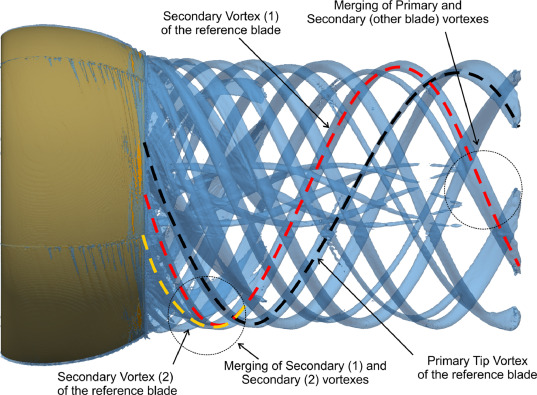
\includegraphics[width=\textwidth]{Figures/Litterature_review/Gaggero_swirl.png}
    \caption{Wake of a ducted RDT with primary and secondary helical vortices, adapted from Gaggero et al.~\cite{Gaggero2023}.}
    \label{fig:rdt_wake_gaggero}
  \end{subfigure}
  \hfill
  \begin{subfigure}[b]{0.45\textwidth}
    \centering
    
\includegraphics[width=\textwidth]{Figures/Litterature_review/Anderson_pump_GV.png}
    \caption{Hubless rim-driven axial pump with downstream guide vanes for swirl recovery, adapted from Andersen~\cite{Andersen2014}.}
    \label{fig:andersen_rdt_vanes}
  \end{subfigure}
  \caption[RDT wake and guide-vane recovery]{Wake structure of rim-driven thrusters and the corresponding guide-vane recovery concept.}
  \label{fig:rdt_wake_and_vanes}
\end{figure}
 
The wake is therefore not a free design variable in the present thesis. It is a fixed input drawn from a single set of RDT simulations, and the comparative ranking of the twenty-four guide-vane configurations is performed against the same wake. The screening result is in this respect conditional on the chosen RDT simulation; the same screening method, applied to a different RDT wake, would be expected to produce a similar Pareto-front shape but a different identification of the optimal vane geometry.
 
\section{Pre-rotation sensitivity of the RPT in pump mode}
\label{sec:lit_prerotation}
 
The most important reason that the residual swirl after the guide vanes is not free to be ``something low'' is the pre-rotation sensitivity of the downstream RPT. Two studies on the same NTNU laboratory RPT model establish this directly. Larsen~\cite{Larsen2019} reports that, in pump mode, no efficiency increase is observed when pre-rotation is added, but that negative pre-rotation (NPR, opposite to the runner rotation) increases the head while positive pre-rotation (PPR, in the runner-rotation direction) decreases it. Jenssen~\cite{Jenssen2020} carried out homogeneous-mixture cavitation simulations of the same machine with imposed forced-vortex pre-rotation profiles at maximum angles of $\pm 20^\circ$ and $\pm 40^\circ$ and reports an asymmetric cavitation response: NPR can reduce the required cavitation number by up to 25\,\% while PPR can increase it by as much as 93\,\%. A small NPR is therefore tolerable or even useful in pump mode; a small PPR of the same magnitude is harmful.
 
This sign-dependent sensitivity is the reason the present master thesis cannot simply minimise a single magnitude metric. The conventional design objective, ``zero swirl at the inlet'', remains the safe baseline, but the comparative ranking in Chapter~\ref{chap:chap5} reports both magnitude and sign of the residual swirl, and the discussion treats a small NPR as a more favourable outcome than a small PPR of the same magnitude. The same observation also limits the extent to which a Francis-turbine guide-vane design tradition~\cite{Brekke2003, Brekke2015} can be transferred to the present problem, because Francis vanes are designed around prescribed pre-rotation that the runner is matched to. In the present case the runner is fixed and the vane row must match the runner rather than the other way round.
 
\section{Swirling flow through $90^\circ$ bends}
\label{sec:lit_bend}
 
The downstream geometry in the Store2Hydro layout includes a $90^\circ$ bend between the guide-vane section and the position of the RPT inlet. This element is not part of the guide-vane design problem in the conventional sense, but it is part of the design \emph{system}, because residual swirl from the vane row interacts with the bend before reaching the RPT. The literature on this interaction is mature in the pipe-flow community but, to the present author's knowledge, has not been brought into the booster--RPT design discussion at all.
 
The fundamental result on plain $90^\circ$ bends is that the curvature imposes a radial pressure gradient across the cross-section that cannot be balanced uniformly by the non-uniform velocity profile, so the flow develops a counter-rotating pair of secondary cells in the cross-stream plane: the Dean vortices, whose strength scales with the Dean number $\mathrm{De} = \mathrm{Re}\sqrt{D_h/2R_c}$~\cite{Dean1927}. The high-Reynolds turbulent regime relevant to the present work has been investigated extensively. Kim, Yadav and Kim~\cite{KimYadavKim2014} performed a benchmark CFD study of the secondary flow in a $90^\circ$ elbow using OpenFOAM and showed that the swirl intensity of the post-bend secondary motion depends strongly on the bend curvature ratio and only weakly on Reynolds number, and that the dissipation downstream of the bend is approximately exponential. A more recent study by Wang et al.~\cite{Wang2025DeanVortex} provides a detailed simulation of Dean-vortex evolution in a turbulent $90^\circ$ pipe bend at curvature ratio $1.25$ and confirms the same qualitative picture, while documenting the extent of the post-bend asymmetry across multiple cross-sections.
 
When the upstream flow already carries swirl, the picture is more complicated. Liu and Vanierschot~\cite{LiuVanierschot2021} review the literature on swirling flow through curved pipes and report that the Dean cells and the upstream swirl interact in a sign-dependent way: depending on whether the swirl rotates with or against one of the Dean cells, that cell is amplified or suppressed, with the corresponding consequence for the post-bend cross-stream velocity profile. Escue and Cui~\cite{EscueCui2010} verify that the SST $k$--$\omega$ model captures the bulk structure of decaying swirling pipe flow but tends to underpredict turbulence anisotropy under strong rotation, which sets a known limit on the accuracy of two-equation RANS in this regime. Within the Store2Hydro project itself, Jenssen~\cite{Jenssen2020} explicitly observed bend-induced separation and an asymmetric cross-stream profile in the original RPT draft-tube geometry, and motivated his choice of velocity-profile boundary condition downstream of the bend with this observation.
 
For the master thesis, two implications follow. First, the post-vane plane is not the only location at which the comparative ranking should be evaluated; planes downstream of the bend must also be reported, because the bend can change the ranking. Second, the sign of the residual swirl entering the bend is a relevant design variable, and the discussion of the screening result in Chapter~\ref{chap:chap5} should retain this distinction explicitly.
 
\section{Cascade closure: solidity, diffusion limits and slip}
\label{sec:lit_cascade}
 
The blade-element method that underlies the parametric guide-vane construction is classical~\cite{Wallis1968} and is reused in this thesis from~\cite{Leonsen2025}. The closure relations needed to translate a target swirl into a vane geometry --- solidity, diffusion-factor limits, and the deviation correction at the trailing edge --- are reviewed only briefly here, because they are well established and are revisited in detail in Chapter~\ref{chap:chap3}.
 
The diffusion-factor limit due to Lieblein, Schwenk and Broderick~\cite{Lieblein1953} ($D_f \lesssim 0.6$) and the de Haller bound on the relative-velocity ratio ($W_2/W_1 \geq 0.72$) are the standard screening tools to flag overloaded blade rows in axial compressor and stator design. For the present application both are exceeded over part of the design span by all configurations on the Pareto front, because the required turning is so large near the inner radius. The two criteria are therefore retained as comparative indicators rather than as design constraints, in line with the practice~\cite{Schnoes2018, Leonsen2025} adopts for highly loaded axial machines.
 
For deviation, Beaubert et al.~\cite{Beaubert2015, Beaubert2016} document the dependence of slip on turning angle, solidity and Reynolds number for swirl-generating vanes in straight pipes, and the project work~\cite{Leonsen2025} produced a CFD-based slip database for the chosen NACA-type profile family that was condensed into a smooth response-surface model. The present master thesis does not develop the slip model further. Instead, it adopts G\"ulich's~\cite{Gulich2010} recommendation that a small fixed built-in trailing-edge correction in the range $4^\circ$--$6^\circ$ is sufficient to compensate for cascade deviation in well-designed pump and stator vanes, and uses $\delta_{\mathrm{TE}} = 6^\circ$ uniformly across all twenty-four configurations. The justification is given in Chapter~\ref{chap:chap4}: aggressive correction following the response-surface prediction at high turning angles increases the suction-side adverse pressure gradient and tends to promote separation, which is undesirable in a screening campaign where the goal is to compare the geometric effects of vane count and chord-control strategy without a confounding slip-correction variable.
 
\section{Numerical framework for swirling internal flows}
\label{sec:lit_cfd}
 
The numerical framework adopted for the screening campaign --- steady RANS in ANSYS CFX with the SST $k$--$\omega$ turbulence model of Menter~\cite{Menter1994} --- is the de-facto standard for hydraulic turbomachinery in industrial CFD. Its known limitations under strong rotation~\cite{EscueCui2010} are summarised above and are revisited in Chapter~\ref{chap:chap3}. Two methodological choices that are specific to this thesis are noted here.
 
The discretisation uncertainty for the unstructured draft-tube domain is estimated using the Grid Convergence Index (GCI) procedure of Celik et al.~\cite{Celik2008}, originally rooted in the work of Roache~\cite{Roache1998}. The procedure is applied to the swirl number at the bend exit, which is the single most sensitive integral output for this domain (Section~\ref{sec:gci_drafttube}). The structured turbomachinery meshes for the rotating RDT and for each guide-vane row are generated with ANSYS TurboGrid and are assessed through bounded mesh-quality metrics rather than through a full triplet-based GCI procedure. The justification, developed in Chapter~\ref{chap:chap4}, is that for structured hexahedral O-grids on isolated blade rows with $y^+ \approx 1$ and bounded skewness/orthogonality, the integral output quantities of interest are weakly sensitive to mesh density above a moderate threshold~\cite{Menter1994}, and a separate triplet-based GCI for each of the twenty-four blade meshes would not be cost-effective.
 
\section{Rotor--stator interaction in compact configurations}
\label{sec:lit_rsi}
 
The compact RDT--GV configuration considered in the master thesis places the rotor and the stator within a fraction of a chord from each other, which is the regime in which rotor--stator interaction (RSI) becomes a primary source of unsteady loading. Brekke's monograph on hydraulic turbines~\cite{Brekke2010, Brekke2015} reviews the historical record of RSI-related vibration and pressure-pulsation problems in Francis machines and provides the order-of-magnitude thresholds that distinguish acceptable from problematic pulsation amplitudes. The classical theoretical framework for the spatial-mode structure of the pulsation field is the Tyler--Sofrin analysis~\cite{Tyler1962}, which decomposes the unsteady pressure field around a rotor--stator stage into circumferential modes of order $m_{k,j} = k Z_r - j Z_s$. The lowest-order mode at the blade-passing frequency ($k=1$) is $m_{\min} = \min_j |Z_r - j Z_s|$, and three regimes of practical relevance follow: when $\gcd(Z_r, Z_s) = 1$ the lowest mode is at least $|Z_r - Z_s|$ and the net axial force on the stator ring approaches zero by circumferential cancellation; when $Z_r = Z_s$, on the other hand, $m_{\min} = 0$ and the lowest mode is the axisymmetric breathing mode, in which all stator vanes are loaded synchronously at the blade-passing frequency.
 
The baseline configuration in the present thesis uses $Z_r = Z_s = 7$, which is, on Tyler--Sofrin grounds, an a priori unfavourable choice. Whether the breathing mode actually dominates the pulsation field in practice depends on the degree of $Z_r$-fold azimuthal symmetry of the incoming RDT wake and on the spanwise matching between rotor and stator, both of which are imperfect. The unsteady analysis in Chapter~\ref{chap:chap5} is constructed precisely to test this question for the Store2Hydro configuration, using a transient simulation, an FFT-based spectral decomposition of the force, torque and pressure monitor signals~\cite{Bergan2018}, and a ring-coherence diagnostic that distinguishes the $m=0$ breathing mode from spinning modes $|m| \geq 1$. The reference amplitude thresholds reported by Egusquiza et al.~\cite{Egusquiza2006} and the wet-natural-frequency considerations from Tanaka and Valentin~\cite{Tanaka2011, Valentin2015} are used to interpret the magnitudes obtained.
 
\section{Identified gap and how this thesis addresses it}
\label{sec:lit_gap}
 
The literature reviewed in this chapter supports the following synthesis. The booster--RPT system is technically attractive, but earlier studies in the field treat the booster and the RPT as two machines without a conditioning element between them. A guide-vane row is the natural response, but the existing CFD evidence covers only two example geometries~\cite{Leonsen2025} and only in a straight-pipe domain. A multi-objective screening tradition exists in the wider turbomachinery community~\cite{Vasilopoulos2019} and has recently been transferred to the marine rim-driven domain~\cite{GaggeroMartinelli2024, Yang2024RDTAppendage}, but has not been used for the hydropower booster--RPT case. The hubless RDT wake imposes a hubless cascade as the only feasible vane geometry. The downstream RPT is sensitive to pre-rotation in a sign-dependent way~\cite{Larsen2019, Jenssen2020}, so the design objective is conditioned residual swirl rather than minimum residual swirl. The $90^\circ$ bend in the downstream geometry interacts non-trivially with residual swirl~\cite{LiuVanierschot2021, KimYadavKim2014, Wang2025DeanVortex}, so the comparative ranking cannot be evaluated only at the post-vane plane. The compact RDT--GV configuration produces unsteady loading whose spatial-mode structure is set by the Tyler--Sofrin combinatorics~\cite{Tyler1962}, and the baseline $Z_r = Z_s = 7$ choice is a priori unfavourable.
 
The master thesis closes the gap that this synthesis identifies by combining (i) a structured screening campaign over twenty-four guide-vane configurations evaluated on a Pareto front, (ii) a CFD domain that includes the $90^\circ$ bend and an extended draft-tube section so that residual swirl is reported both immediately downstream of the vanes and after the bend, and (iii) a transient simulation of the baseline configuration analysed under the Tyler--Sofrin framework. The theoretical apparatus needed to interpret the screening output is developed in Chapter~\ref{chap:chap3}, and the methodology is described in Chapter~\ref{chap:chap4}.
 
\clearpage
 

% Xia et al.\ investigated numerically how inlet and outlet boundary conditions influence confined turbulent swirling flow and showed that the predicted flow field is sensitive to these choices in different ways. Their results indicate that the detailed shape of the inlet velocity profiles is of secondary importance if the mean axial, radial and azimuthal velocity components are preserved separately, whereas the ratio between radial and axial inlet velocity has a much stronger influence on the downstream flow structure and recirculation behaviour. They therefore argued that reliable simulations of swirling flows require not only a correct swirl level at inlet, but also a realistic representation of the radial inflow component. For the outlet, they found that the boundary condition mainly affects the solution close to the numerical exit, while its influence decays upstream if the outlet is placed sufficiently far downstream. This supports the general CFD strategy of extending the downstream domain and placing the numerical outlet away from the region of interest when studying strongly swirling internal flows, so that the outlet condition does not artificially modify the wake development or swirl-recovery process \cite{Xia1997}. 

